\documentclass[10pt,twocolumn]{article}
\usepackage[margin=0.75in]{geometry}
\usepackage[T1]{fontenc}
\usepackage{lmodern,amsmath,amssymb,booktabs,graphicx,hyperref}
\usepackage{microtype}
\hypersetup{colorlinks=true,urlcolor=blue,linkcolor=blue}
\title{BrickPlan 1.0: Certified Assembly-Order Diagnostics\\for Future Feasibility and Recovery}
\author{Release manuscript}
\date{September 30, 2026}
\begin{document}
\maketitle
\begin{abstract}
An assembly action can be locally legal and geometrically correct while forcing
later removal. End-to-end success alone does not identify this failure mode.
BrickPlan 1.0 connects interactive assembly outcomes to exact future-feasibility
labels in a tractable, explicitly restricted workcell. The release contains two
original LDraw subassemblies, eight episodes, and 26 diagnostic responses.
Exhaustive enumeration covers 58,616 reachable states and 568,648 directed
transitions. Seven diagnostic dimensions measure dead-end choices, supplied-plan
conflict prediction, plan survival, regret, recovery, replanning efficiency, and
counterfactual consistency. Every repair start requires at least three removals.
A shared HTTP executor supports model clients, human practice, and original-mesh
3D replay. Software controls validate the implementation; no language-model or
human performance is reported. This small known-pose release establishes an
auditable measurement contract, not broad long-horizon generalization.
\end{abstract}

\section{Motivation and research question}
Brick assembly requires choosing an order as well as a final configuration.
Closing a region too early can obstruct a later insertion even when the closure
is at its correct final pose. A useful planning diagnostic must distinguish
this event from an invalid immediate action, a pose-estimation error, or an
incomplete response.

Existing studies motivate this distinction but report different quantities.
LEGO-Puzzles studies multistep reasoning and planning~\cite{legopuzzles};
PhyBlock evaluates physical planning and understanding~\cite{phyblock};
Brick-Composer examines fine-grained part selection and pose prediction~\cite{composer}.
Their planning, selection, and joint step metrics are not interchangeable
episode success rates. Interactive disassembly and reconstruction also precede
this work, including LTRON~\cite{ltron} and instruction-memory approaches such as
InstructioNet~\cite{instructionet}. We do not claim that interaction, removal,
or long task sequences are new in themselves.

The operational question is: \emph{Does an agent choose actions that preserve
completion feasibility, and can it detect and repair a loss at a justified cost?}
Version 1.0 deliberately controls placement geometry to isolate order selection.
Its contribution is an executable diagnostic contract linking local choices
and recovery to certified costs, with explicit missing-response and censoring
rules. Establishing external validity and model discrimination remains future
experimental work.

\section{Workcell and task construction}
\subsection{Declared action domain}
Each task contains a connected, clamped fixed base, a finite inventory, calibrated
sites, and a visible target. Every site preserves an original source pose.
\texttt{attach} and \texttt{detach} translate one part along its declared straight
path. The workcell includes transfer to an external magazine; motion outside
the audited insertion/extraction segment and hand/tool geometry are not modeled.
All accepted states remain connected to the fixed base through audited stud
connections, treated as rigid holds. The support plate in the renderer denotes
this abstract fixture.

The executor uses only current occupancy, path blockers, and connector support.
It receives no goal or optimal policy when deciding local legality. It therefore
accepts a legal closure even if that choice causes later rework. All public sites
remain selectable; there is no next-step action mask. The goal requires exact
site occupancy. Equivalent inventory instances share a part type and color,
while public instance/site IDs are stable within an episode and permuted by seed.

Each structural attempt costs one action, including failures. Inspection and
diagnosis have separate quotas, and finishing costs no structural attempt.
The browser supports free camera inspection and exploded target reference.
Actual assembly states are never exploded. This interface is for structured
practice and review; matched vision-only model/human evaluation is not implemented.

\subsection{Geometric qualification}
Original LDraw triangles are used for display. Collision qualification uses
versioned closed proxy meshes with a 0.25 LDraw-unit inset and 0.002-unit guard.
Endpoints are checked for intersection and containment. A clear path is certified
by separating swept bounds or a distance cover: translation distance is
1-Lipschitz, so a midpoint clearance larger than half the interval length plus
the guard covers the whole interval. A triangle-intersection witness certifies
a blocked path. Unresolved intervals remain \texttt{UNKNOWN} and exclude a case
from this release.

One upstream 3022 proxy has a missing triangular stud-cap face. The repair checks
its location and boundary against the original source, then fills that face
without moving vertices. Source/render geometry is unchanged. These are guarded
floating-point certificates over specified meshes and paths, not unrestricted
motion or clutch-force guarantees.

\begin{table}[t]
\centering\small
\caption{Frozen structures. Both derive from the same LEGO 31027 provenance group.}
\begin{tabular}{lrr}
\toprule
Property & Roadster & Kart\\
\midrule
Source parts & 37 & 25\\
Fixed / movable & 20 / 17 & 7 / 18\\
Reachable states & 14,012 & 44,604\\
Directed transitions & 131,824 & 436,824\\
Optimal full actions & 17 & 18\\
Mandatory chain (parts) & 4 & 4\\
Minimum repair removals & 3 & 3\\
Endpoint pairs & 666 & 300\\
Motion pairs (blocked) & 612 (30) & 432 (19)\\
Unknown geometry & 0 & 0\\
\bottomrule
\end{tabular}
\label{tab:cases}
\end{table}

\begin{figure*}[t]
\centering
\begin{minipage}{.24\textwidth}\centering
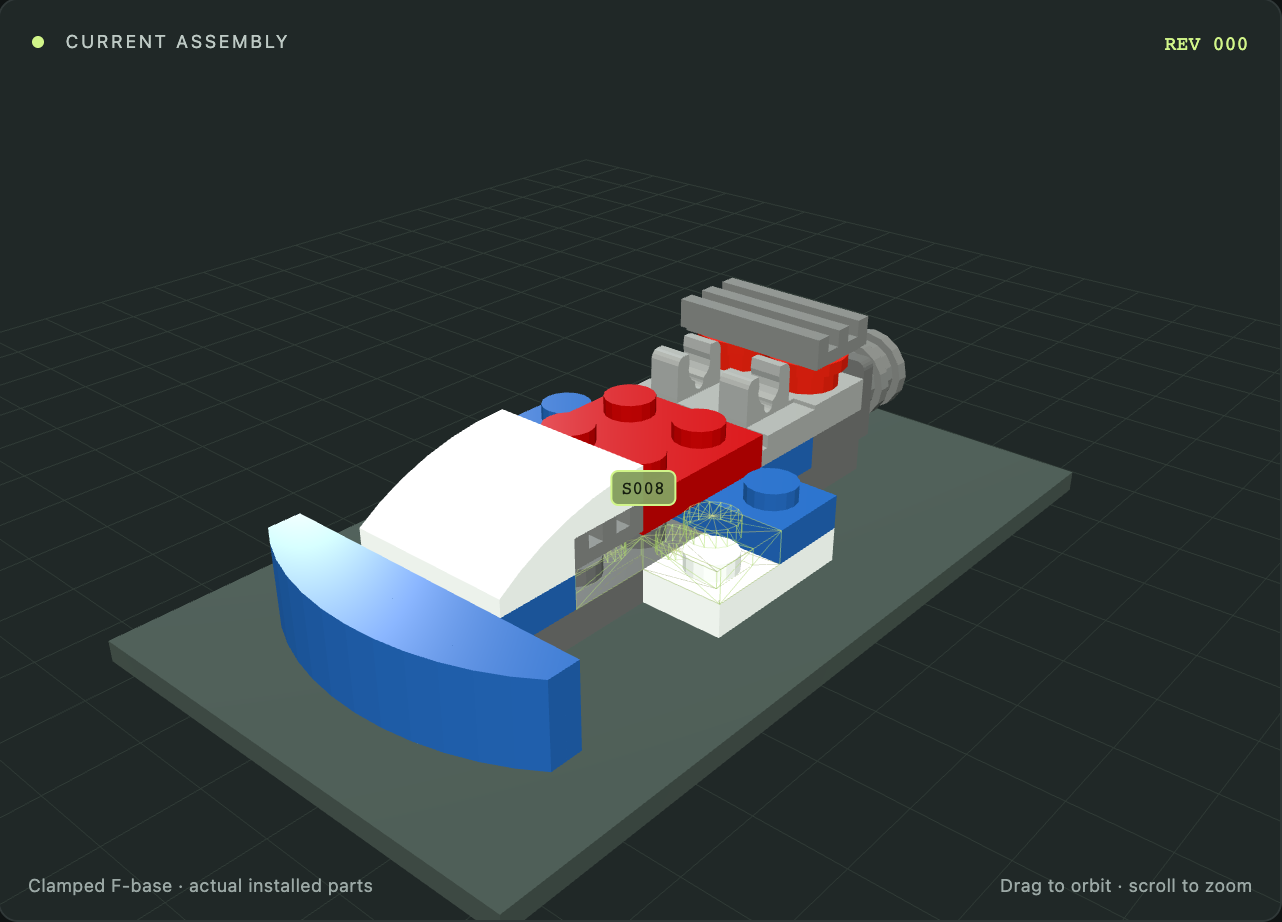
\includegraphics[width=\linewidth]{figures/repair-0.png}\\
\small (a) Repair start: $D^*=3$.
\end{minipage}\hfill
\begin{minipage}{.24\textwidth}\centering
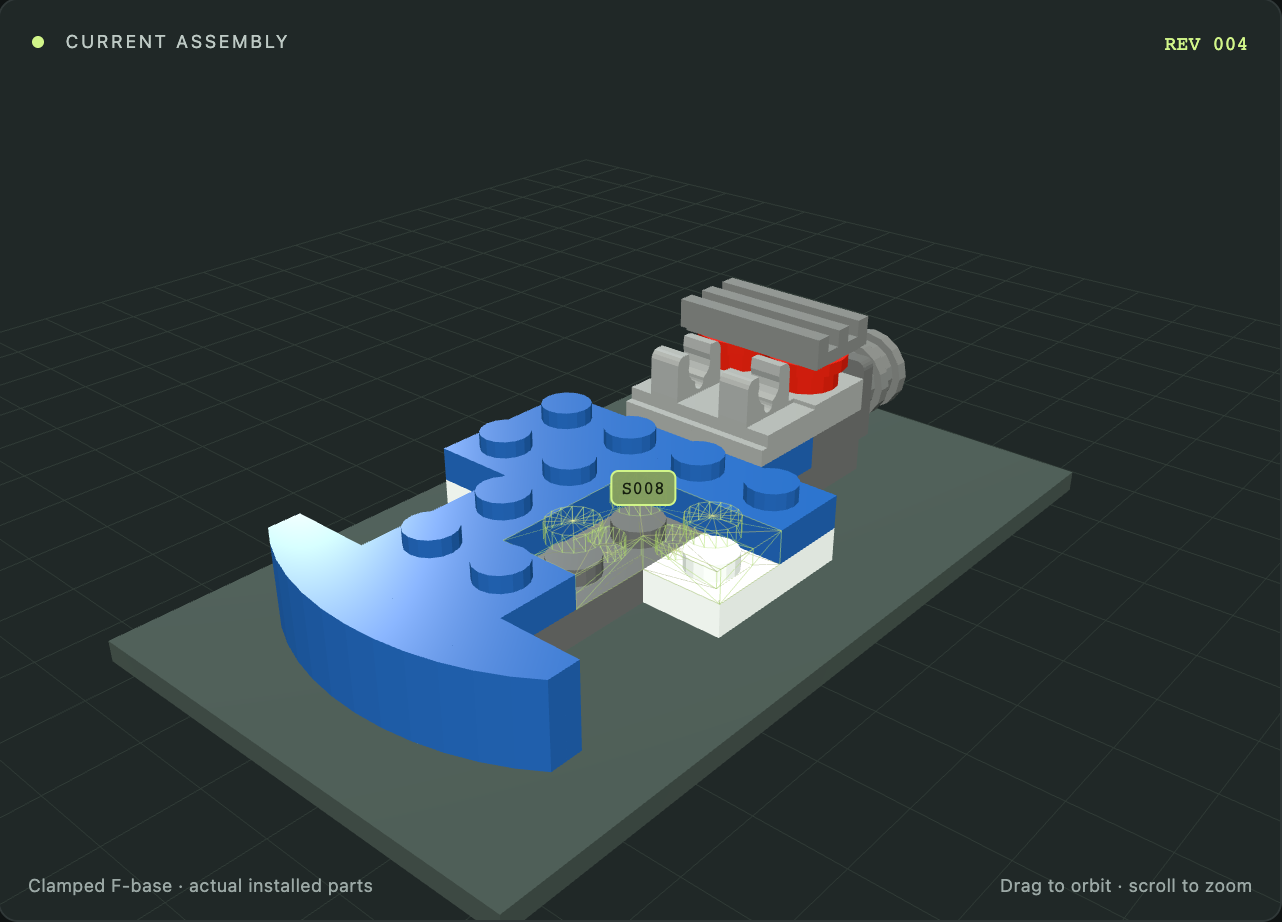
\includegraphics[width=\linewidth]{figures/repair-1.png}\\
\small (b) Remove three closures.
\end{minipage}\hfill
\begin{minipage}{.24\textwidth}\centering
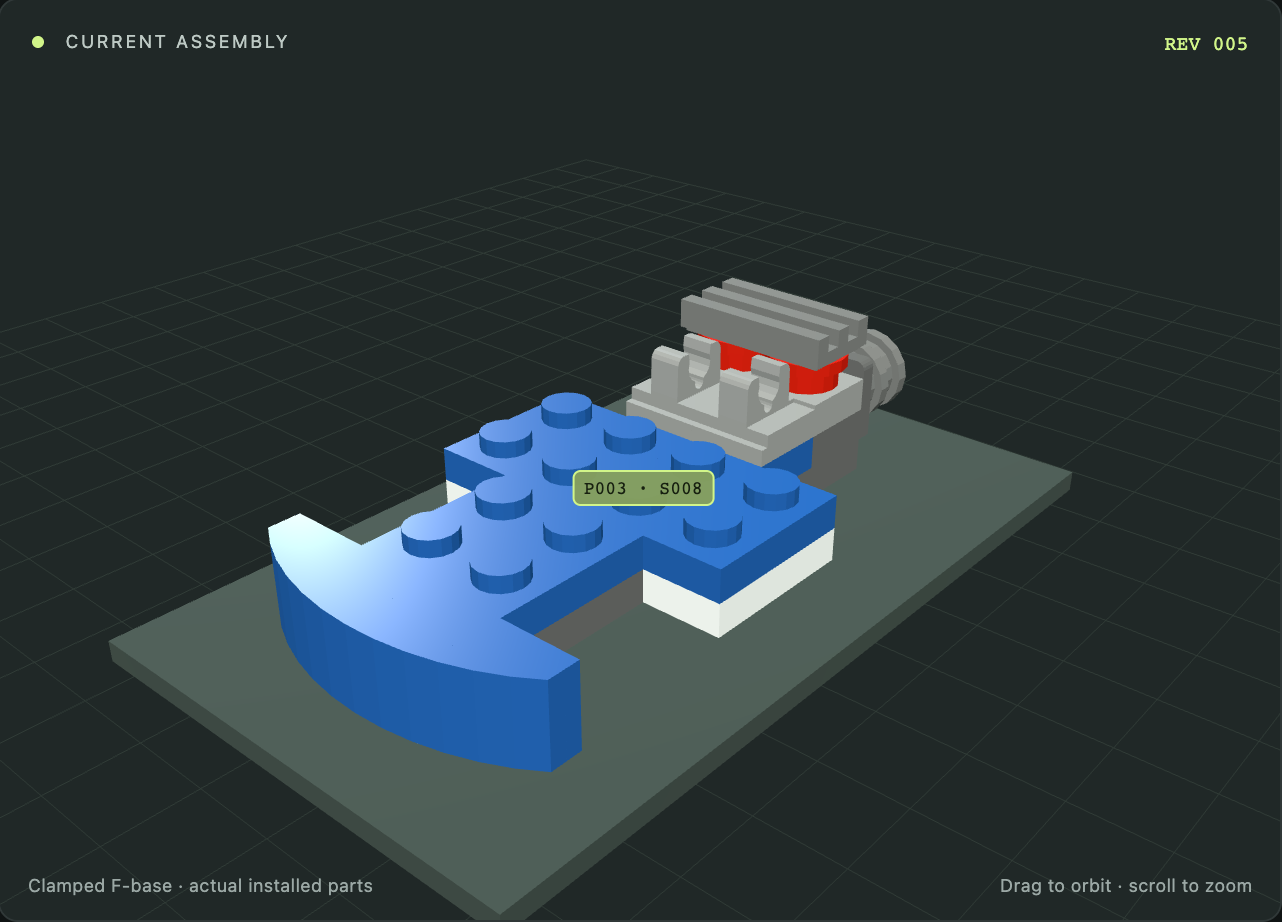
\includegraphics[width=\linewidth]{figures/repair-2.png}\\
\small (c) Insert P003 at S008.
\end{minipage}\hfill
\begin{minipage}{.24\textwidth}\centering
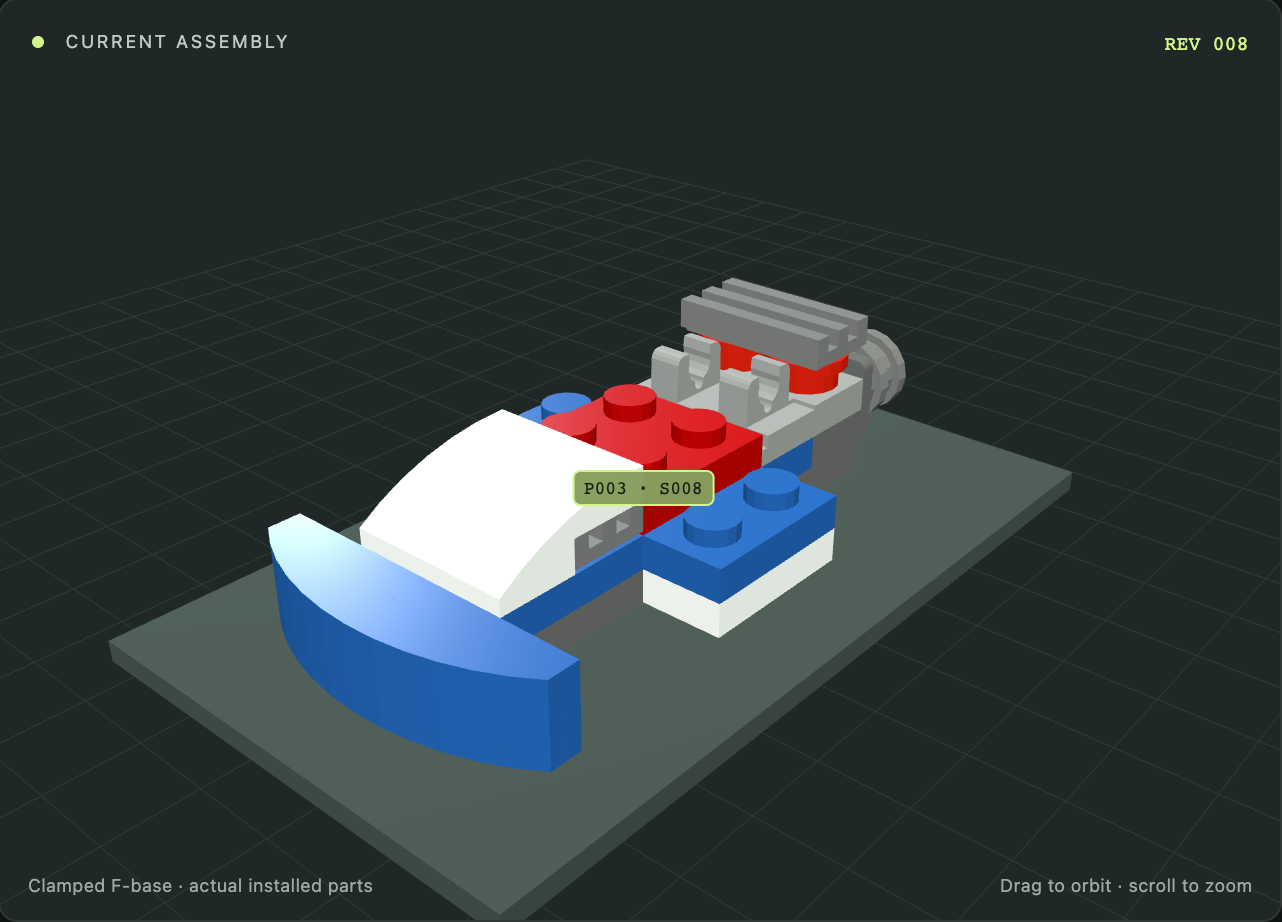
\includegraphics[width=\linewidth]{figures/repair-3.png}\\
\small (d) Restore and complete.
\end{minipage}
\caption{Authoritative kart repair replay, seed 31. The replay removes P005,
P008, and P018 before inserting the missing interior part.
Three removals and four attachments complete the target in seven structural
actions, matching the exact optimum. The wireframe in earlier frames denotes
the empty calibrated site, not a floating installed brick. These are original
source meshes rendered from real executor states; no model performance is implied.
Frame revisions are 0, 4, 5, and 8 because diagnosis uses a revision but no
structural action.}
\label{fig:repair}
\end{figure*}

\subsection{Finite-state certification}
Let $s$ denote occupied mutable sites and $g$ the exact target. Exhaustive search
enumerates the reachable component. Every legal structural edge has a verified
reverse edge. Goal-rooted breadth-first search gives the exact remaining action
cost $C^*(s,g)$. Every table is checked against Bellman inequalities, unique
zero-cost termination, and a decreasing successor at each nonterminal state.
Certificates include geometry, transition, task, and cost hashes.

Let $\Delta=|g|-|s|$. For successful one-part unit-cost actions, attachments
minus detachments equal $\Delta$. Consequently the minimum detach count is
\[
 D^*(s,g)=\frac{C^*(s,g)-\Delta}{2}.
\]
No-undo feasibility $V^+(s,g)$ holds exactly when $s\subseteq g$ and
$C^*(s,g)=\Delta$. Remaining-budget feasibility is
$V_B(s,g,b)=[C^*(s,g)\le b]$. A no-undo dead end is recoverable with removal;
it is not absolute impossibility in the reversible graph.

\subsection{Frozen episodes and probes}
Each structure supplies full build, checkpoint continuation, injected repair,
and matched healthy continuation episodes. Checkpoints follow three legal
attachments. Repair starts are reachable and have $D^*=3$. Healthy controls
match installed count and inherit the repair budget, preventing a diagnosis
shortcut from the displayed budget. Both are publicly labeled continuation.
The default budget is $C^*+\max(4,\lceil C^*/2\rceil)$.

Two choice probes provide currently legal candidates, with tight remaining
budgets equal to the optimal cost. Sixteen lookahead probes use first-conflict
distances 1, 2, 4, and 8, with an executable matched-length control per structure
and distance. Eight counterfactual responses form one switch pair and one
invariance pair per structure. Randomizing IDs and presentation order does not
increase the number of independent structures.

\section{Seven diagnostic dimensions}
\paragraph{Dead-end choice rate.}
Among valid assigned legal choices with a feasible predecessor, measure the
fraction whose successor loses $V^+$, and separately the fraction losing
$V_B(s',g,b-1)$. Missing/invalid responses are reported separately, along with
avoidance over all assigned probes. A model cannot obtain full avoidance credit
by abstaining.

\paragraph{Lookahead.}
Before execution, predict the exact first failing index of a supplied plan or
\texttt{null} if all its actions execute. Report exact accuracy, conflict recall,
false alarms, and coverage by distance. In this release the conflict dependency
depth is one; larger distances include intervening legal attachments. Thus these
probes measure conflict-prediction horizon, not internal search depth. An
executable control need not preserve global completion feasibility.

\paragraph{Plan survival.}
Record the first attempted-action index losing each feasibility predicate.
Recovery does not erase this event. At time $t$, report known survivors,
first-loss outcomes, and unresolved early stops, with bounds
$S_{\rm lower}(t)=N_{\rm alive}(t)/N$ and
$S_{\rm upper}(t)=(N_{\rm alive}(t)+N_{\rm unresolved}(t))/N$.
Stratify by structure, mode, reference length, and budget. A completed successful
run is absorbing; an abandoned run is not assumed to survive forever.

\paragraph{Regret.}
For completed successful runs, action regret is attempted actions minus
$C^*(s_0,g)$; detach regret is successful detach operations minus $D^*(s_0,g)$.
Failed runs receive \texttt{null} regret and explicit consumed costs. Under this
action domain, action regret equals twice detach regret plus failed attempts.
The two cost measures should not be treated as independent latent abilities.

\paragraph{Recovery.}
Score the first explicit \texttt{needsRework} diagnosis before any successful
structural change to the injected checkpoint. Earlier failed attempts are
allowed and separately flagged. Report detection recall, precision, matched
healthy false alarms, completion, and joint detection/completion. Later
diagnosis spam cannot replace the first answer.

\paragraph{Replanning efficiency.}
For successful repair suffixes, report attempted actions, removals, distinct
removed instances, excess costs, failed attempts, and the first action reducing
$D^*$. Conditional efficiency must accompany recovery completion rate.
Repeated removal counts repeatedly as work but once per distinct part.

\paragraph{Counterfactual consistency.}
Hold the state, inventory, sites, paths, and two offered closures fixed; change
the visible future goal. Both closures are required in every paired target.
Certify conditional costs $Q^*(s,a,g)=1+C^*(T(s,a),g)$.
Switch pairs have different minimizing offered actions; invariance pairs retain
the same minimizer. Score joint correctness before raw switching or invariance.
The minimum is over offered candidates, not all possible actions: an interior
insertion may be globally better. Answers are normalized to physical actions
after independent candidate-position permutations.

\section{Validation and experimental status}
\subsection{Evaluation settings}
Complete success at the frozen budget is the headline outcome; the seven
dimensions form a profile, not a weighted leaderboard score. Policy observations
exclude source instruction indices, blockers, future costs, feasibility labels,
and witnesses. Private certificate files are for auditors, not model inputs.
HTTP requests are revision checked and idempotent. Terminal-only review, exact
trajectory replay, atomic journals, and explicit selection among repeated runs
make evaluation traceable.

\begin{table}[t]
\centering\small
\caption{Measured software validation controls. These are not VLM baselines.}
\begin{tabular}{lrr}
\toprule
Controller & Complete & Repair\\
\midrule
Privileged optimal oracle & 8/8 & 2/2\\
Fault + optimal recovery & 8/8 & 2/2\\
Trap + attach only & 2/8 & 0/2\\
\bottomrule
\end{tabular}
\label{tab:controls}
\end{table}

Fourteen adversarial tests cover all frozen goal tables, tampered proofs, missing
responses, failed trajectories, censoring, wrong switching, identity equivalence,
diagnosis timing, budgets, and replay. A separate actual HTTP test completes
eight episodes and 26 probe responses, verifies persistence and restart,
rejects duplicate answers, then collects and scores the run. Browser tests
complete one full build with a charged incompatible-part attempt and one
three-detach repair, then exercise replay, exports, probe identity, and desktop
and mobile layouts. Figure~\ref{fig:repair} uses that certified repair session.

\begin{table}[t]
\centering\small
\caption{Empirical study slots. No model or human measurements are available.}
\begin{tabular}{ll}
\toprule
Study condition & Status\\
\midrule
Model, stepwise structured policy & Not evaluated\\
Same model, explicit planning policy & Not evaluated\\
Human structured protocol & Not evaluated\\
Matched image-only protocol & Not implemented\\
\bottomrule
\end{tabular}
\end{table}

Before a model study, preregister exact model/version, prompt, context and token
budgets, reasoning settings, observations, seeds, costs, retry handling, and
run-selection rules. Software controls establish internal implementation
behavior; they do not demonstrate population-level discrimination or a human
advantage.

\section{Limitations and next validation target}
This release contains two related structures from one source kit. Full optimal
lengths of 17 and 18 lie in the proposed D1 range; the longest mandatory chain
contains four parts and three edges. It does not establish 64--256-action planning
or independence from memorized topology. Lookahead distance is explicitly
separated from causal depth. No statistical maximum reasoning horizon is inferred.

Calibrated sites and rigid stud support remove pose estimation and dynamics.
Alternative insertion directions, simultaneous multi-part movement, free rotation,
grasp geometry, clutch force, gravity-induced failure, and physical construction
have not been validated. Certificates apply only to the declared motion domain
and proxy geometry. A broader release should vary provenance, dependency depth,
true competing plans, and repair severity, while preserving complete certificates
where tractable. Real model and human measurements must then test whether these
diagnostics explain failures beyond local action errors.

\begin{thebibliography}{9}\small
\bibitem{legopuzzles} LEGO-Puzzles. arXiv:2503.19990, version 4.
\url{https://arxiv.org/html/2503.19990v4}.
\bibitem{phyblock} PhyBlock. arXiv:2506.08708, version 2.
\url{https://arxiv.org/html/2506.08708v2}.
\bibitem{composer} Brick-Composer. arXiv:2606.05445, version 1.
\url{https://arxiv.org/html/2606.05445v1}.
\bibitem{ltron} LTRON / Break and Make. arXiv:2207.13738.
\url{https://arxiv.org/abs/2207.13738}.
\bibitem{instructionet} InstructioNet. arXiv:2410.01111, version 1.
\url{https://arxiv.org/html/2410.01111v1}.
\end{thebibliography}
\end{document}
